\message{ !name(RNA-seq_intro.tex)}\documentclass{beamer}

\mode<presentation>
{
 \usetheme{CambridgeUS}
 \usecolortheme{seagull}
}
\setbeamertemplate{navigation symbols}{}
\usepackage[english]{babel}
\usepackage{times}
\usepackage[T1]{fontenc}
\usepackage[applemac]{inputenc}
\usepackage{amsmath}

\title[RNA-sequencing]
{Characterizing transcriptomes using ngs data}

%\subtitle
%{} % (optional)

\author[] % (optional, use only with lots of authors)
{T.~K�llman}

\institute[Scilife lab] % (optional, but mostly needed)
{
  BILS/Scilife Lab/Uppsala University\\}

\date[20150917] % (optional)
{Sep. 2015}

\subject{Talks}

\pgfdeclareimage[height=3.5ex,width=2\baselineskip]{institut-logo}{Images/BILS-logo.pdf}
%\pgfdeclareimage[height=1.3cm]{uni}{Images/BILS-logo.pdf}
\logo{\pgfuseimage{uni}}
\setbeamertemplate{footline}{\raisebox{-2ex}{\pgfuseimage{institut-logo}}
  \usebeamerfont{date in head/foot}\insertshortdate{}\hfill
  \usebeamertemplate{navigation symbols}\hfill
  \insertframenumber{}/\inserttotalframenumber}
\setbeamertemplate{sidebar right}{}

\begin{document}

\message{ !name(RNA-seq_intro.tex) !offset(-3) }

\begin{frame}
\titlepage
\end{frame}

\begin{frame}
\frametitle{Outline}
\tableofcontents
\end{frame}

\section{The transcriptome}

\begin{frame}
\frametitle{The Central Dogma}
\begin{center}
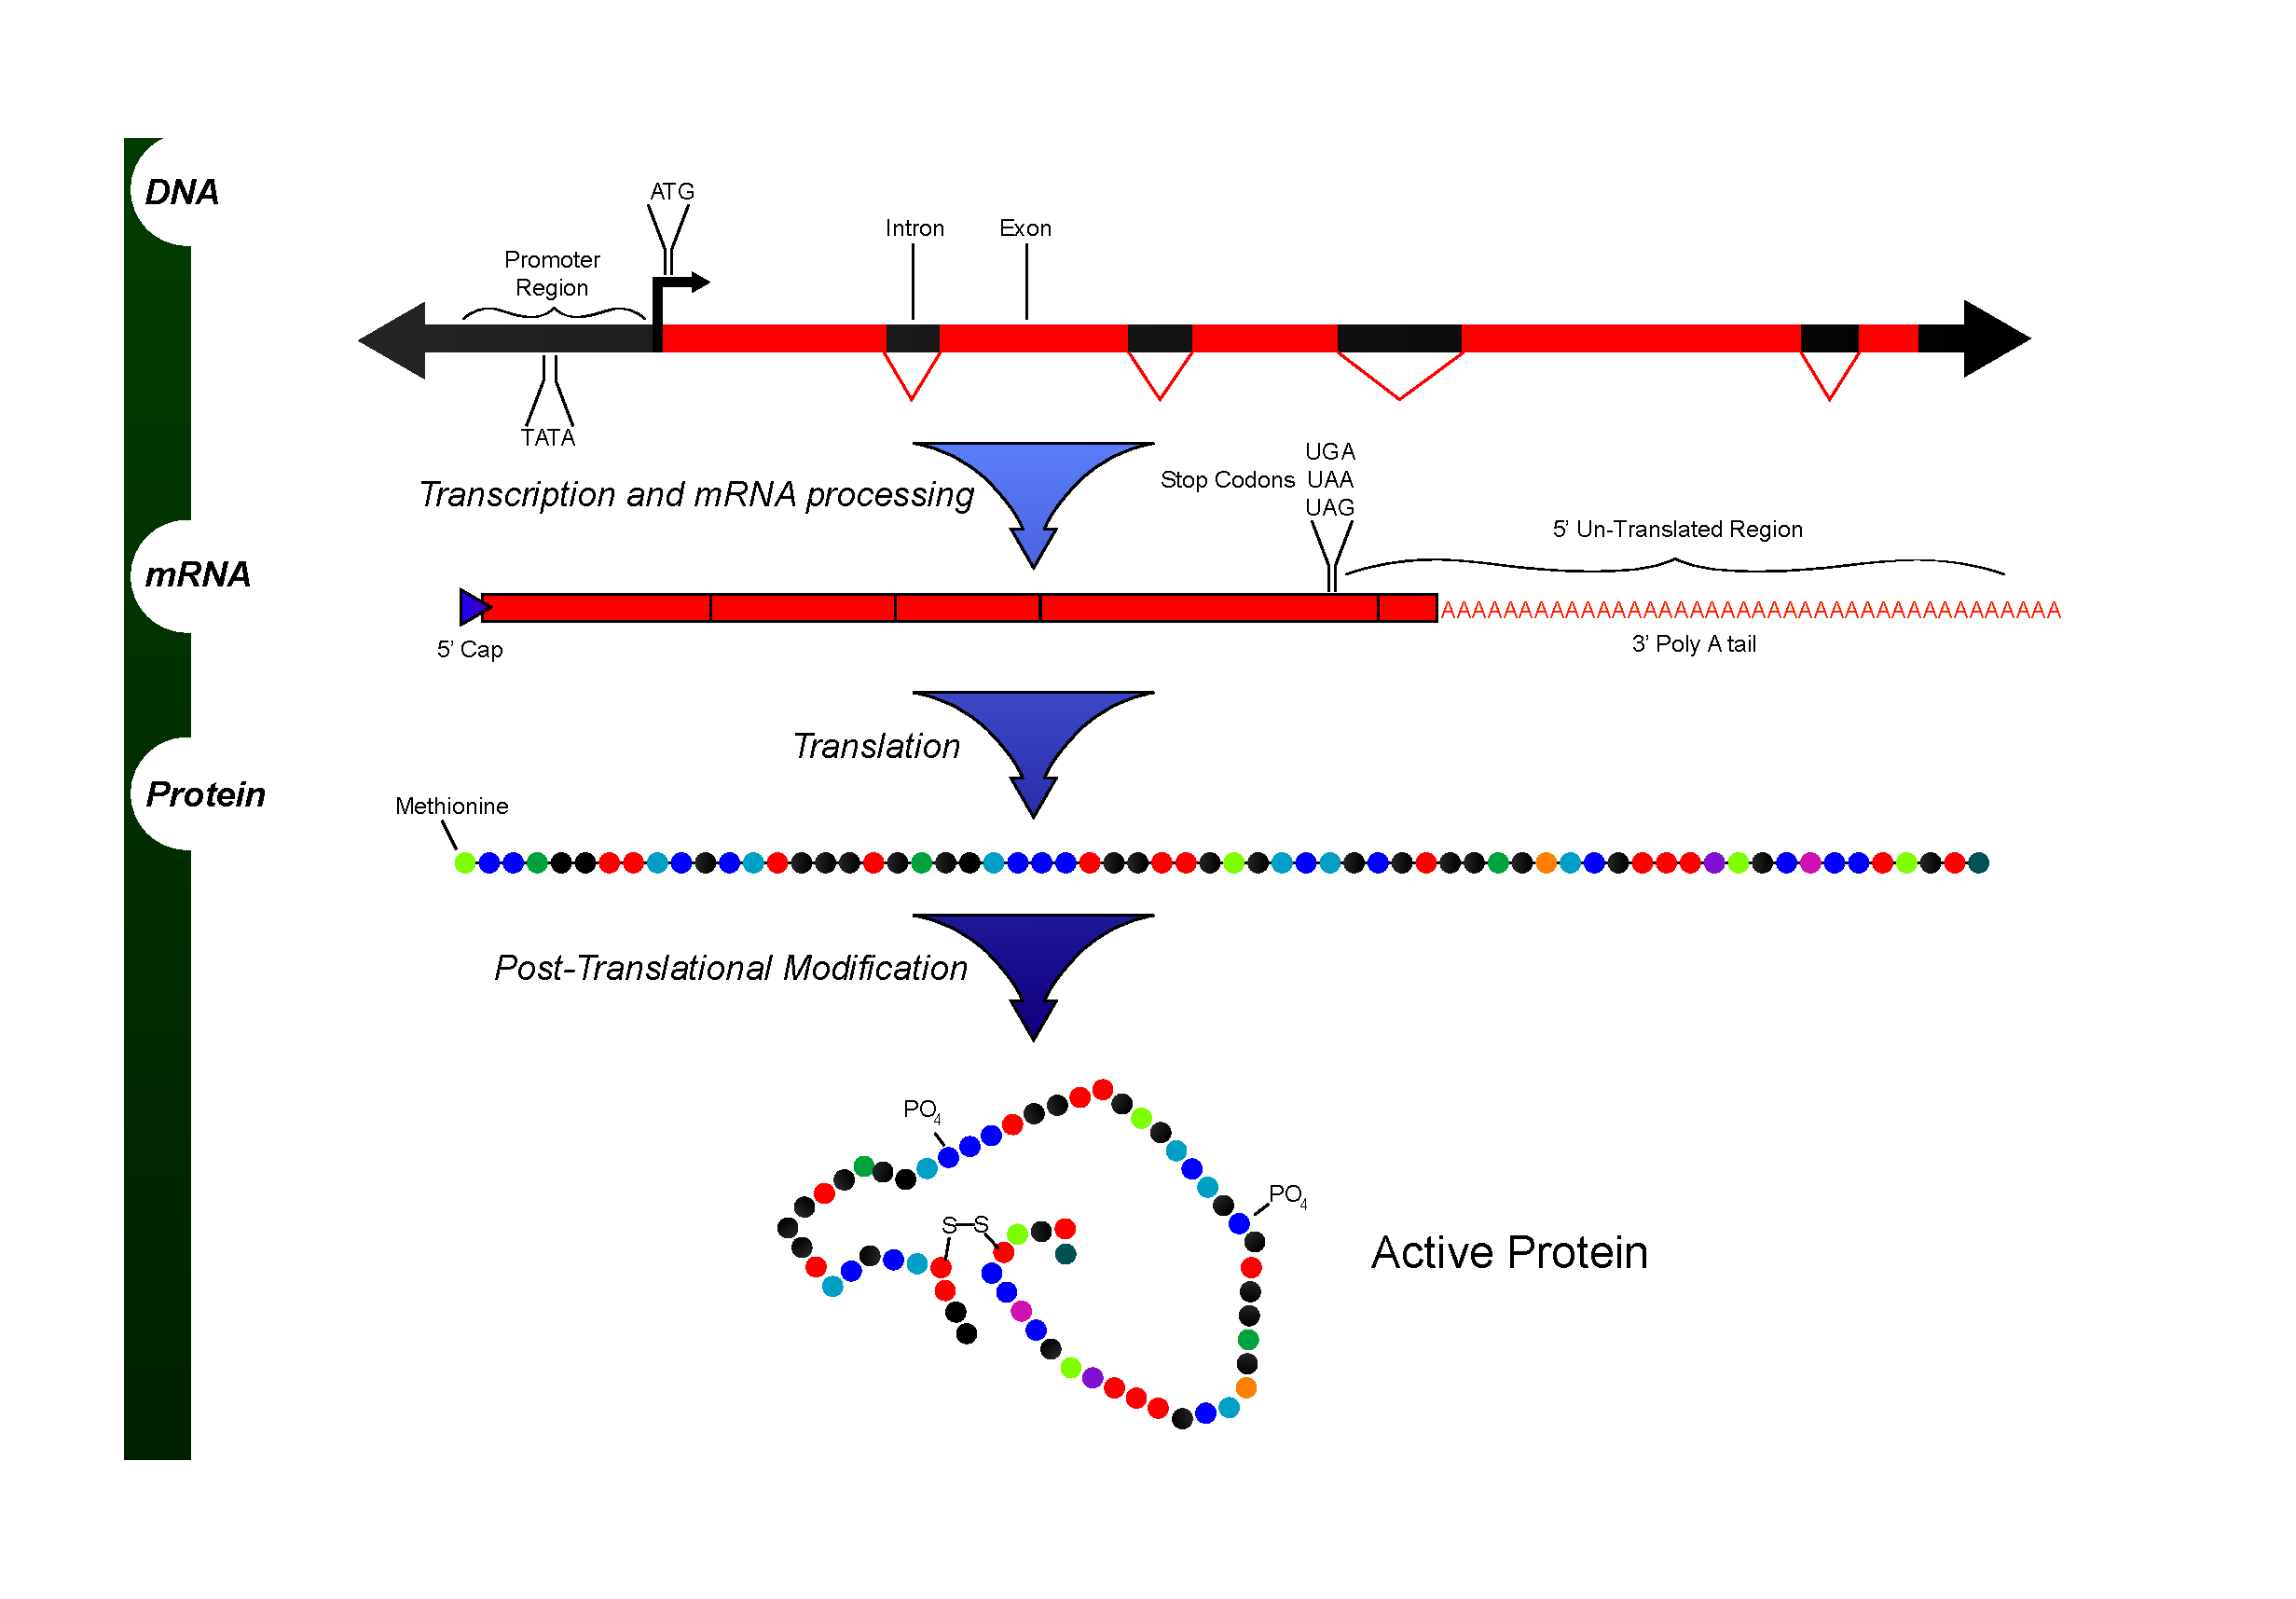
\includegraphics[width=10cm]{Images/Dogma.pdf}
\end{center}
\end{frame}

\begin{frame}
\frametitle{A more complex view}
\begin{center}
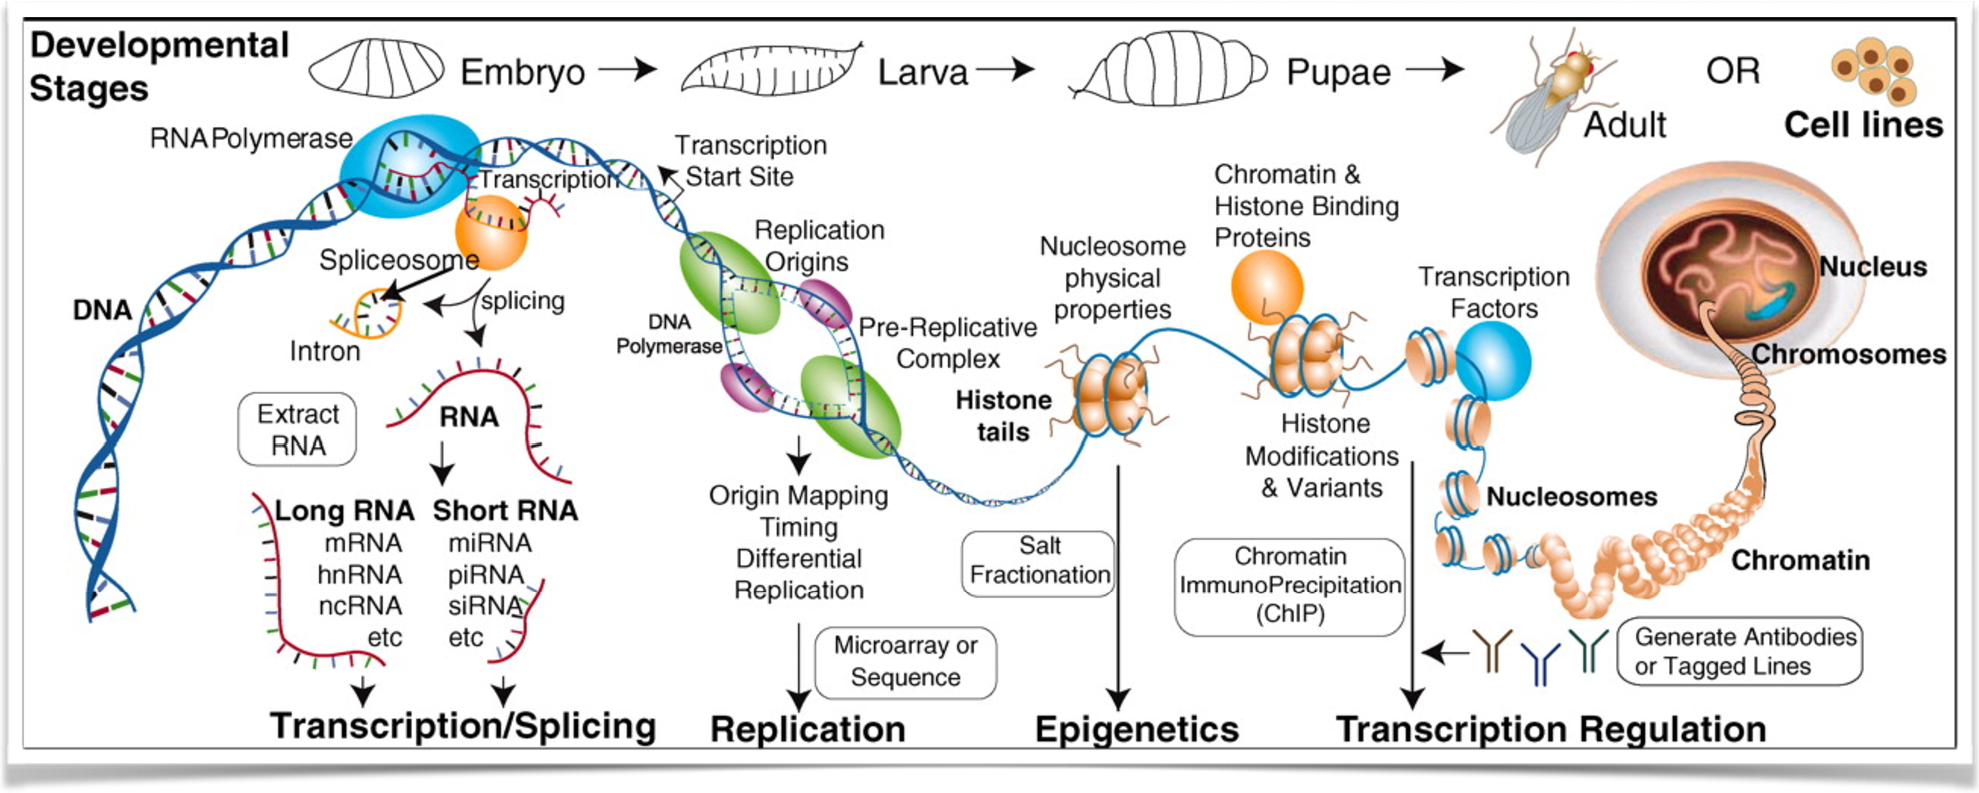
\includegraphics[width=12cm]{Images/TranscriptomeComplex.pdf}
\end{center}
\end{frame}

\begin{frame}
\frametitle{Transcriptomes vs genomes}
\begin{itemize}
\item
Dynamic, not the same over tissues and time points
\item
Smaller sequence space
\item
Less repetitive (but large gene families can be found)
\item
Fairly stable in size? (\textit{eg.} 2-4 fold change among eukaryotes, whereas genome size can vary 1000-fold)
\item
Genes are often expressed in multiple different splice-variants
\item
RNA often from only one strand
\end{itemize}
\end{frame}

\section{RNA sequence technologies}

\begin{frame}
\frametitle{NGS data}
\centering
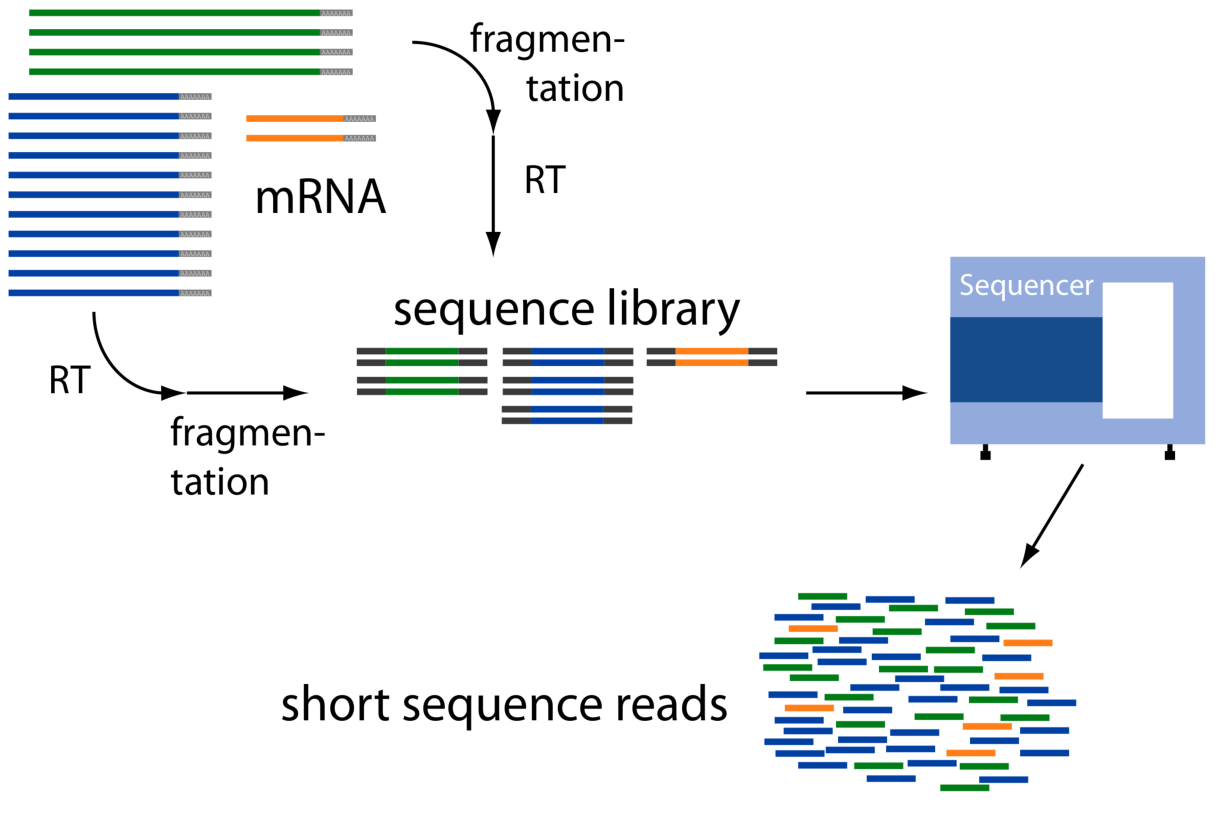
\includegraphics[width=10cm]{Images/RNA-seq.pdf}
\end{frame}

\begin{frame}
\frametitle{Machine output}
\centering
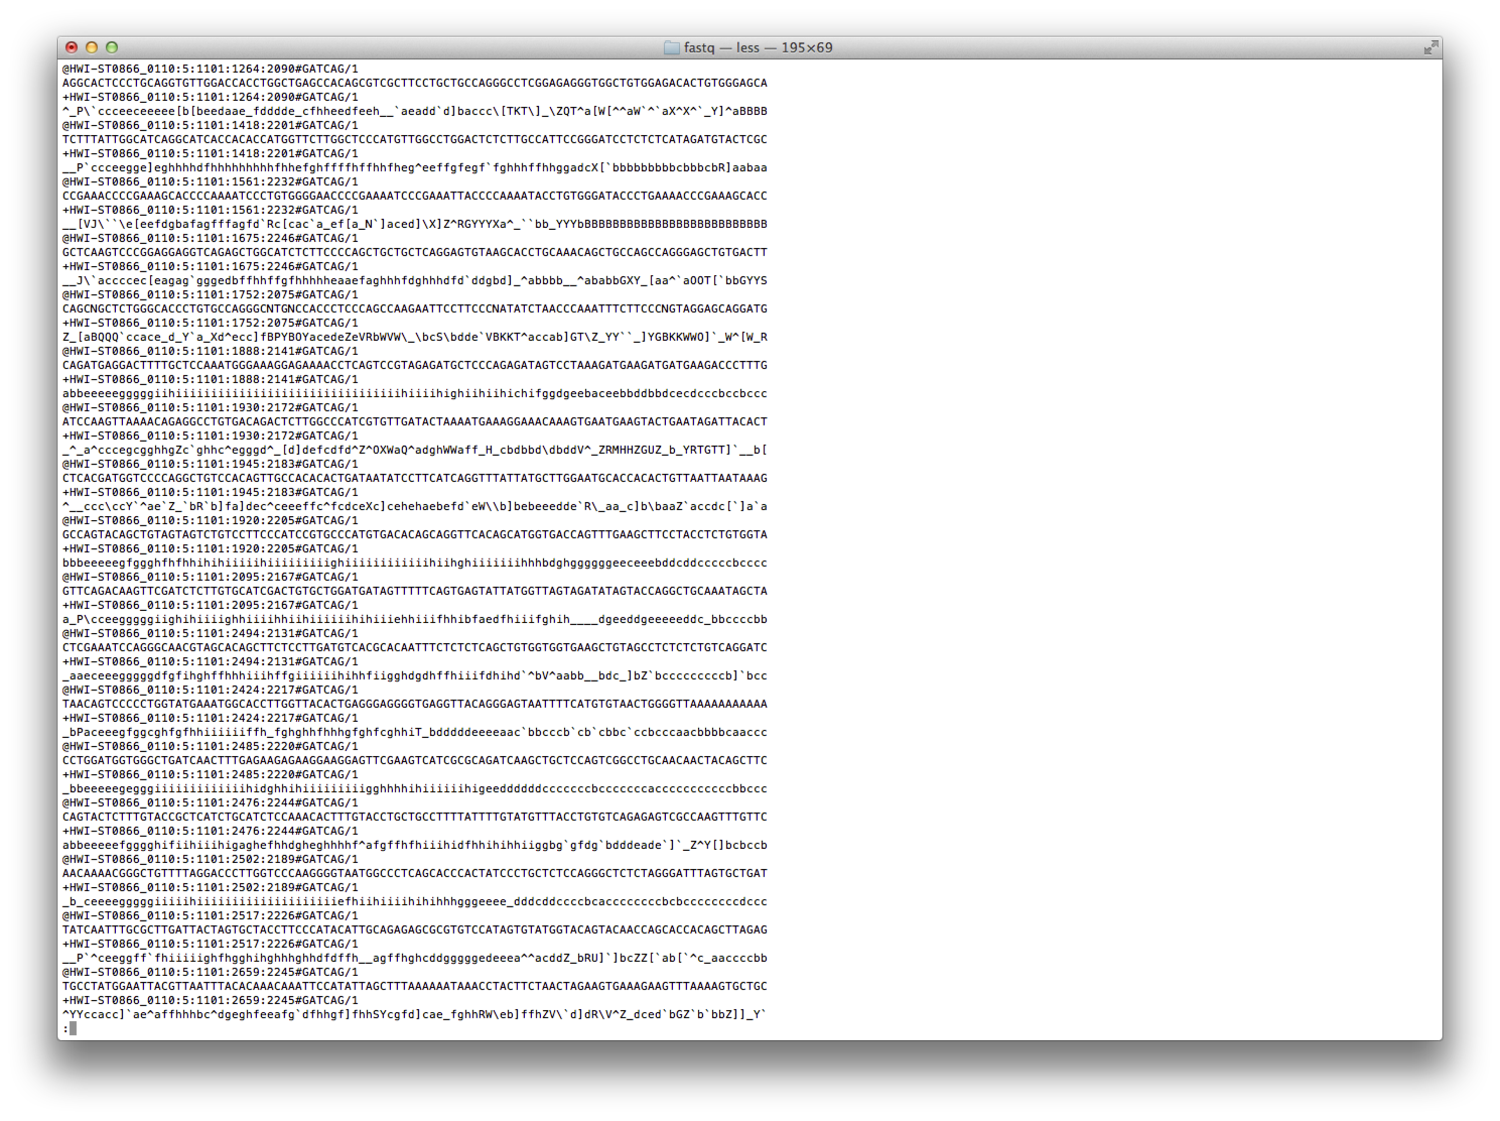
\includegraphics[width=10cm]{Images/fastqless.pdf}
\end{frame}

\begin{frame}
\frametitle{Machine output}
\centering
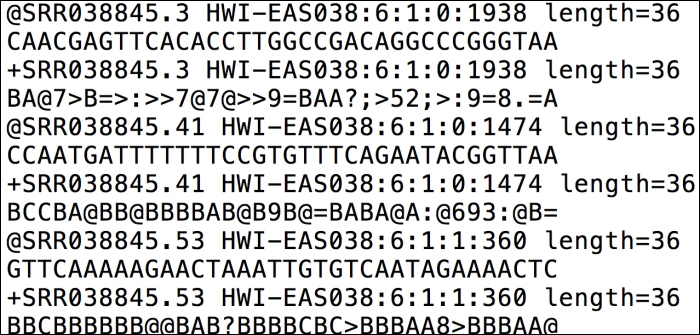
\includegraphics[width=10cm]{Images/fastq36.jpg}
\end{frame}

\begin{frame}
\frametitle{Sequence quality}
\begin{itemize}
\item
Phred quality scores: Q = -10 x log P (High Q = high probability of the base being correct
\item
A Phred quality score of 20 to a base, means that the base is called incorrectly in 1 out of 100 times.
\end{itemize}
\begin{center}
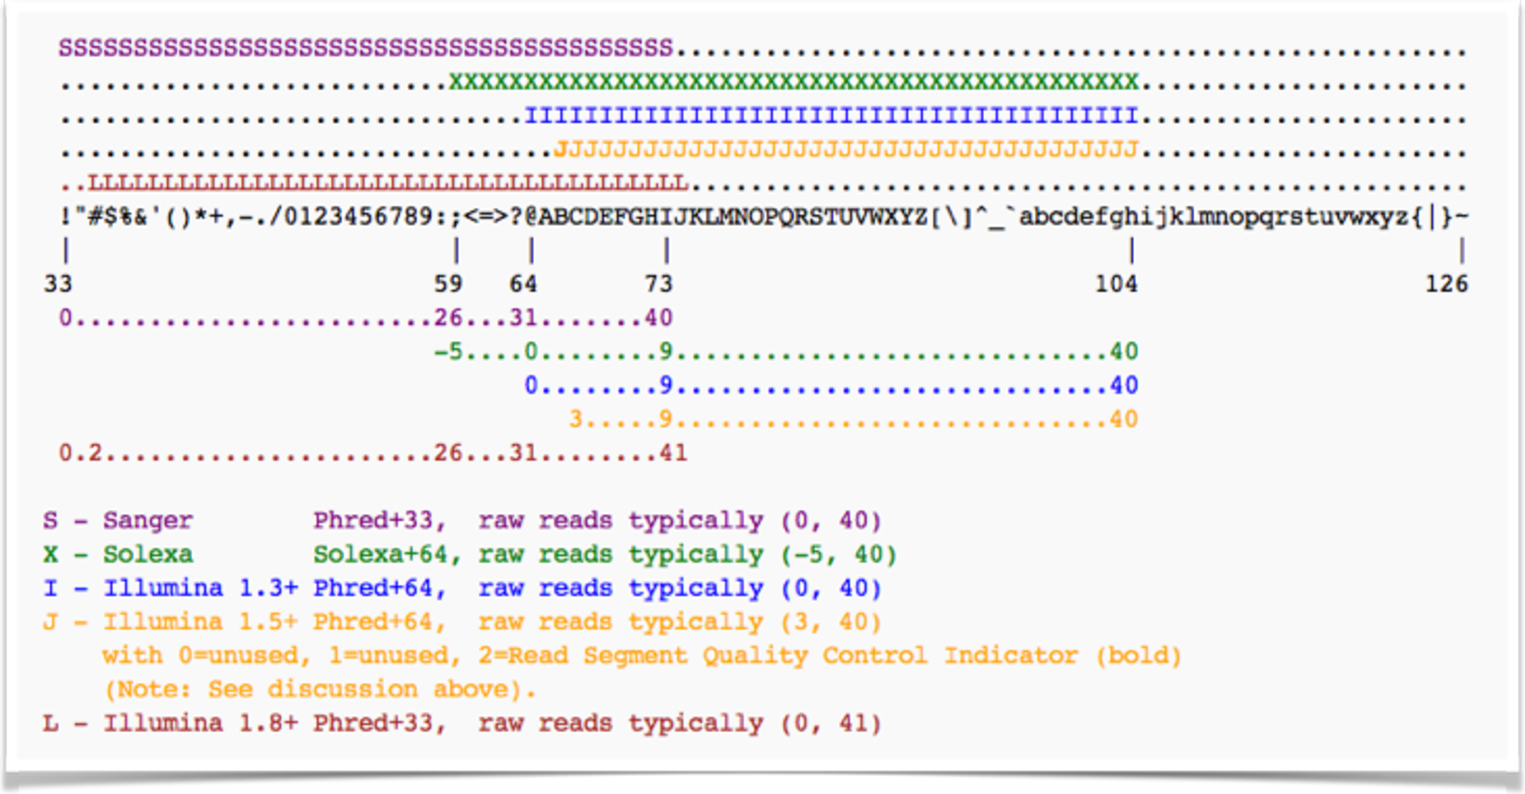
\includegraphics[width=8cm]{Images/fastq.pdf}
\end{center}
\end{frame}

\begin{frame}
\frametitle{Pair-end (PE) sequencing}
\centering
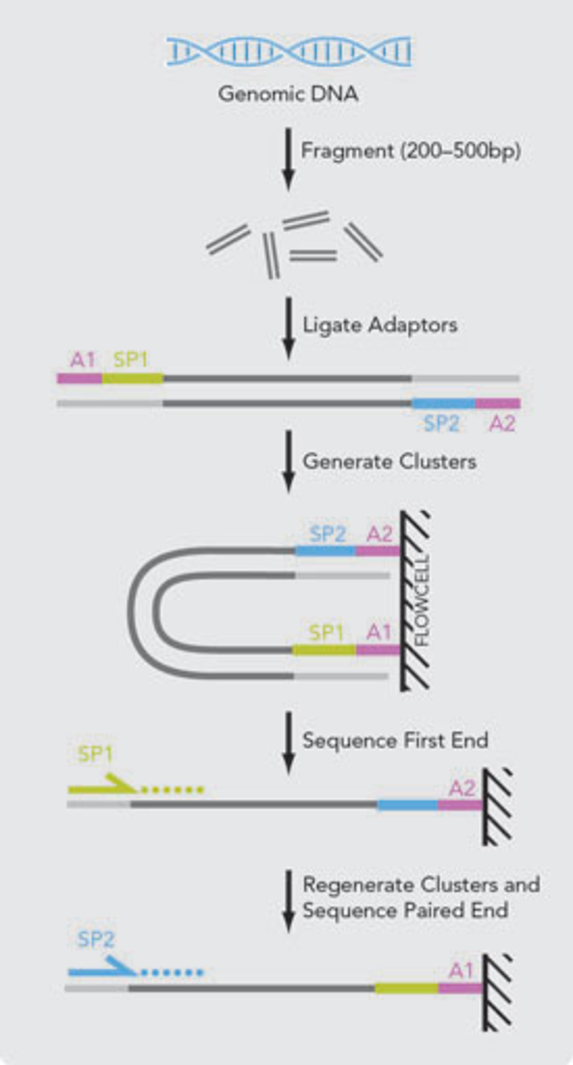
\includegraphics[width=4cm]{Images/PE1.pdf}
\end{frame}

\begin{frame}
\frametitle{Pair-end reads}
\begin{block}{File format}
\begin{itemize}
\item
Two files are created
\item
The order in files identical and naming of reads are the same with the exception of the end
\item
The way of naming reads are changing over time so the read names depend on software version
\end{itemize}
\end{block}
\centering
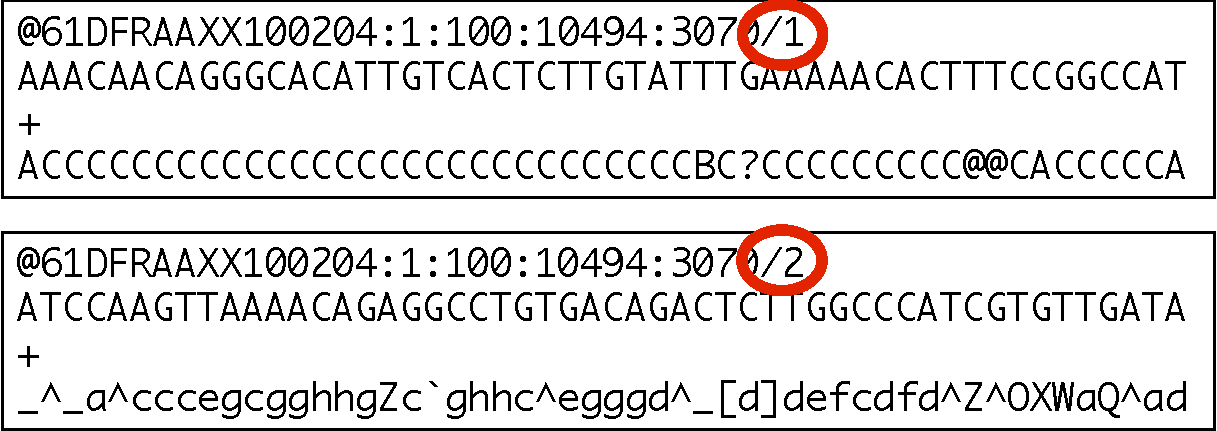
\includegraphics[width=8cm]{Images/twofastq.pdf}
\end{frame}

\begin{frame}
\frametitle{Pair-end data}
\centering
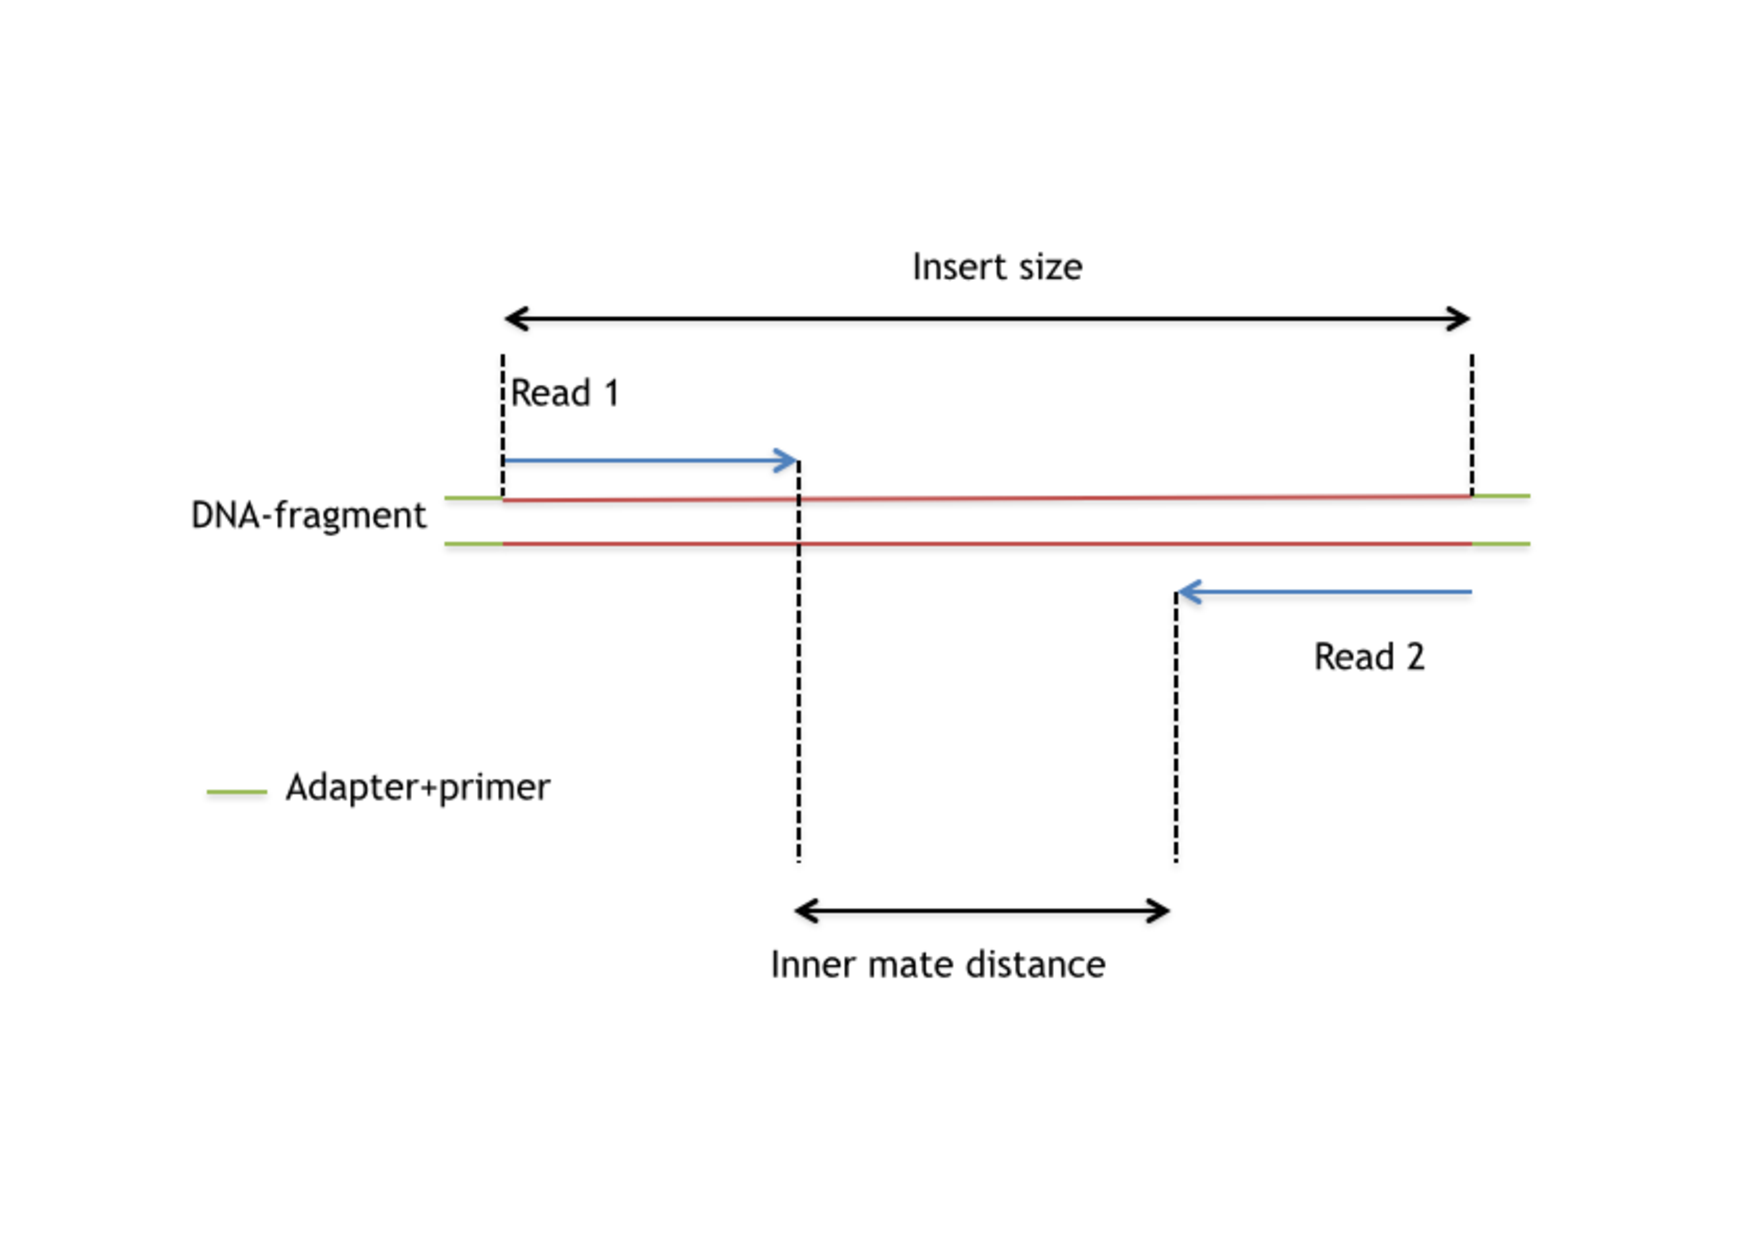
\includegraphics[width=12cm]{Images/PE2.pdf}
\end{frame}

\begin{frame}
\frametitle{Stranded or not}
\centering
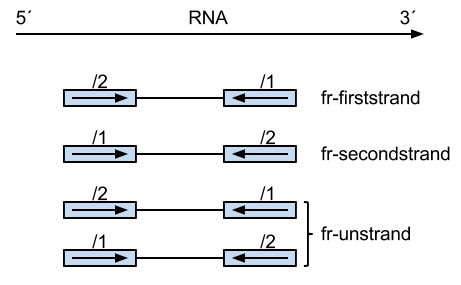
\includegraphics[width=10cm]{Images/Stranded.png}
\end{frame}

\begin{frame}
\frametitle{Basic quality control of raw reads}
\begin{center}
\begin{itemize}
\item
FastQC
\end{itemize}
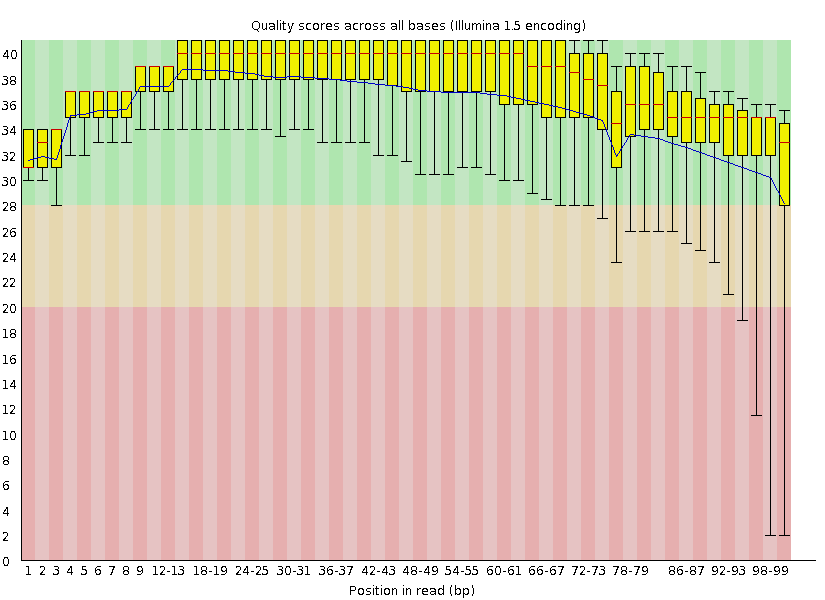
\includegraphics[width=8cm]{Images/per_base_quality.png}
\end{center}
\end{frame}

\begin{frame}
\frametitle{Basic quality control of raw reads}
\begin{center}
\begin{itemize}
\item
FastQC
\end{itemize}
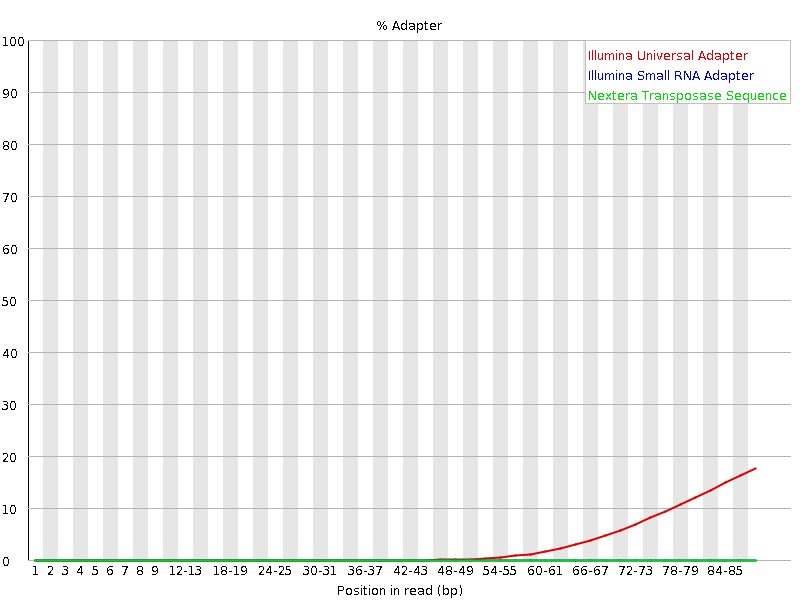
\includegraphics[width=8cm]{Images/adapter_content.png}
\end{center}
\end{frame}

\begin{frame}
\frametitle{Basic quality control of raw reads}
\begin{center}
\begin{itemize}
\item
RNA-seq is not random sample from the genome eg. GC content might be different
\item
Highly expressed genes can be frequent and create warnings in quality controls that assumes whole genome data
\item
Random hexamer in cDNA synthesis might create 'biases' in base frequencies in the beginning of reads
\end{itemize}
\end{center}
\end{frame}

\section{RNA-seq analysis}

\begin{frame}
\frametitle{Two main routes for analysis}
\centering
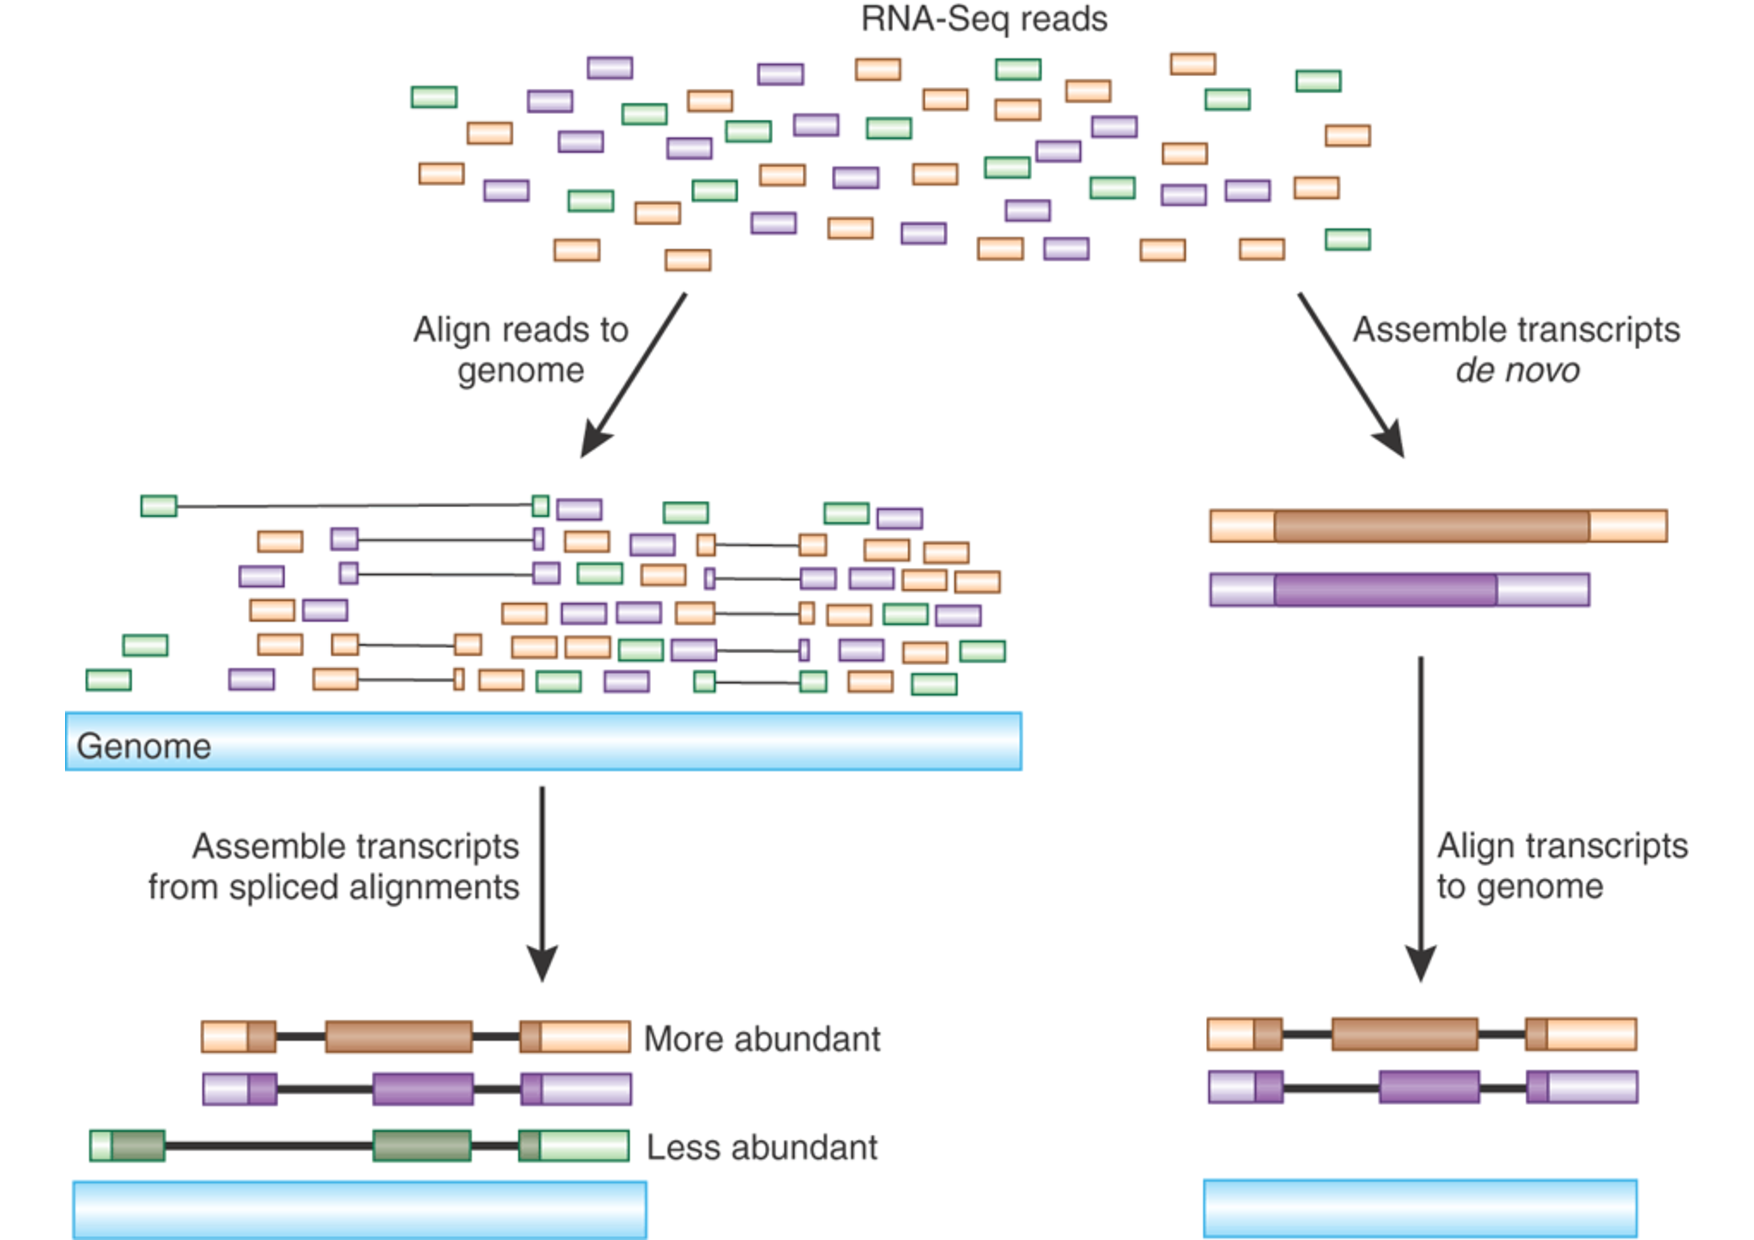
\includegraphics[width=8cm]{Images/advancingRNAseq.pdf}
  \\{\tiny{Haas \& Zody (2010), Nature Biotechnology 28, 421--423}}
\end{frame}

\subsection{Mapping based approach}

\begin{frame}
\frametitle{Aligning short reads from RNA to genomes}
\begin{center}
\begin{itemize}
\item
If available map to the genome sequence
\item
If no genome sequence one can also map to transcriptome reference
\item
Make use of available genome annotation (GTF, GFF, BED files)
\end{itemize}
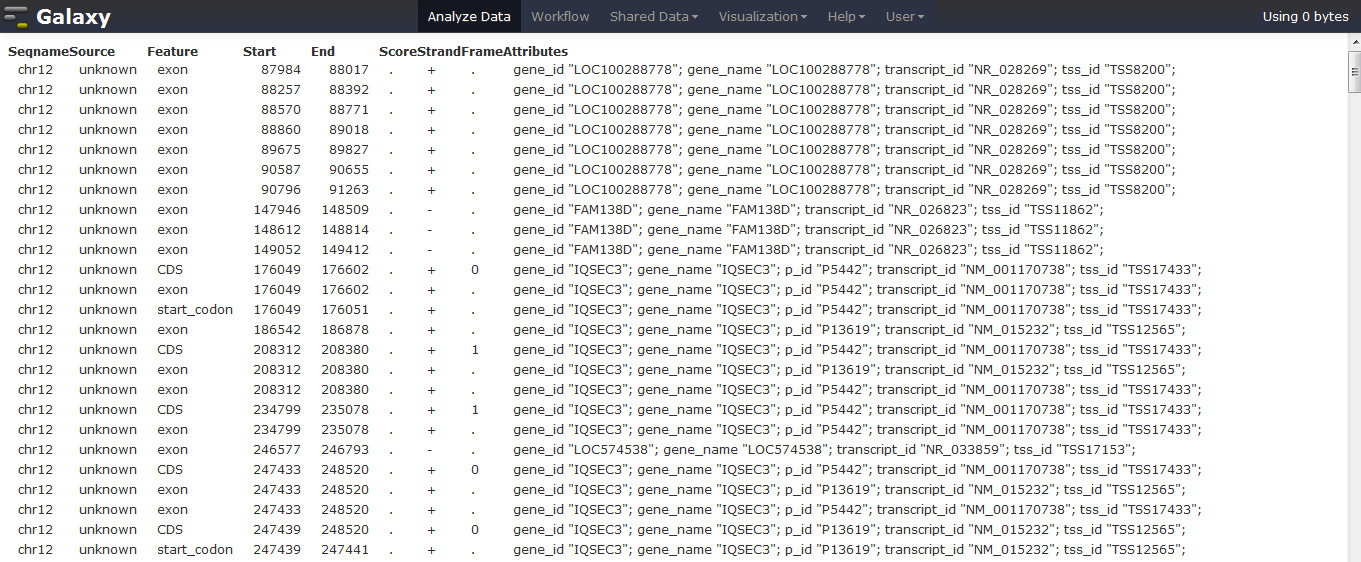
\includegraphics[width=10cm]{Images/gtf.png}
\end{center}
\end{frame}

\begin{frame}
\frametitle{Aligning short reads from RNA to genomes}
\begin{center}
\begin{itemize}
\item
Large number of programs available: Star, Tophat, Subread etc
\item
Important feature: Allow for spliced mapping
\end{itemize}
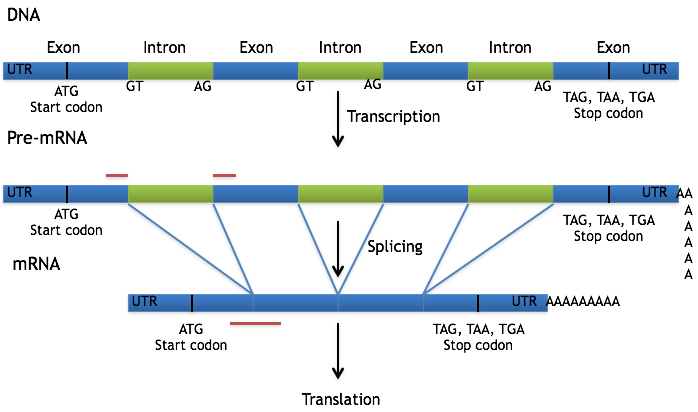
\includegraphics[width=10cm]{Images/SplicedReads.png}
\end{center}
\end{frame}

\begin{frame}
\frametitle{Aligning short reads from RNA to genomes}
\begin{center}
\begin{itemize}
\item
After mapping perform QC of the output
\end{itemize}
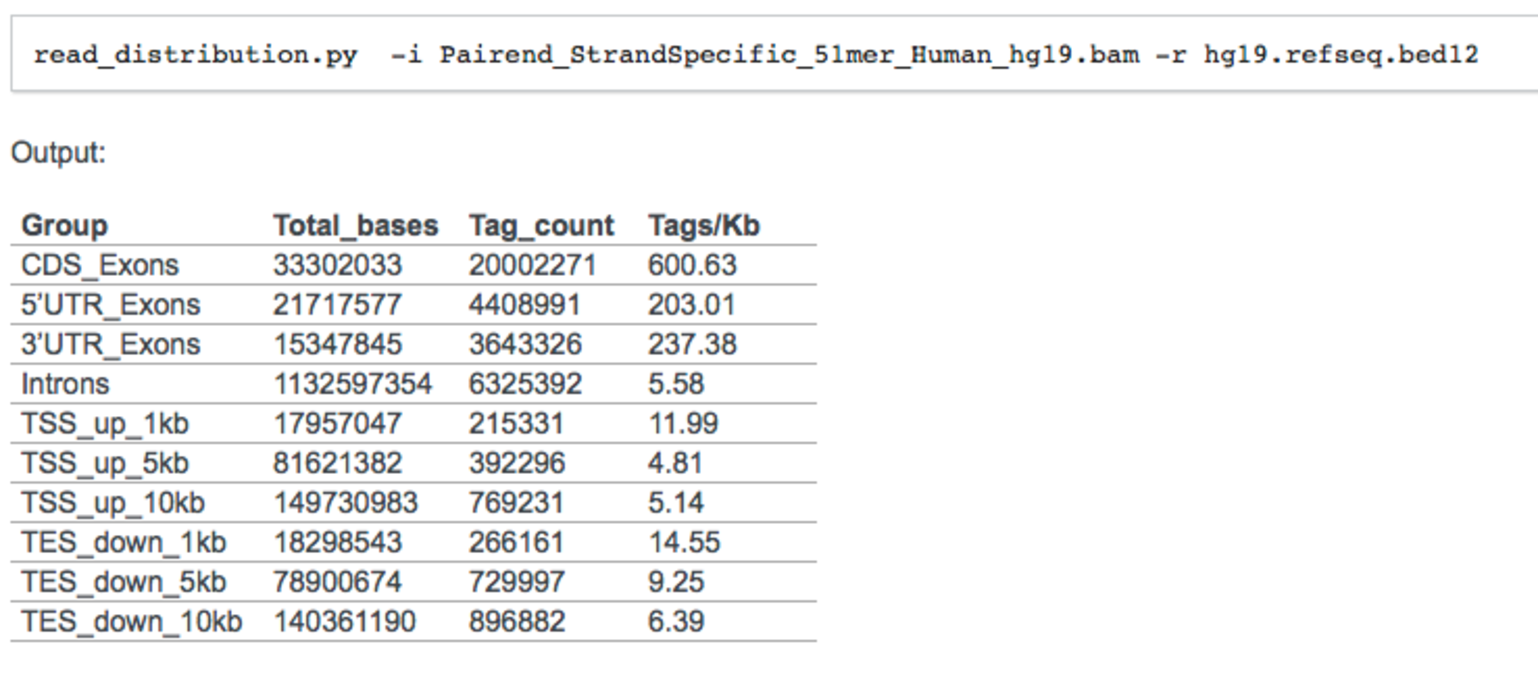
\includegraphics[width=10cm]{Images/read-dist.pdf}
\end{center}
\end{frame}

\begin{frame}
\frametitle{Example workflow}
\begin{columns}
\column{5cm}
\begin{itemize}
\item
Tophat: Aligns reads to genome (allows for spliced read mapping)
\item
Cufflinks: Extract transcripts from spliced read alignments
\item
Cuffmerge: Merge results from multiple Cufflinks results
\item
Cuffdiff: Detect differential gene expression
\end{itemize}
\column{6cm}
\centering
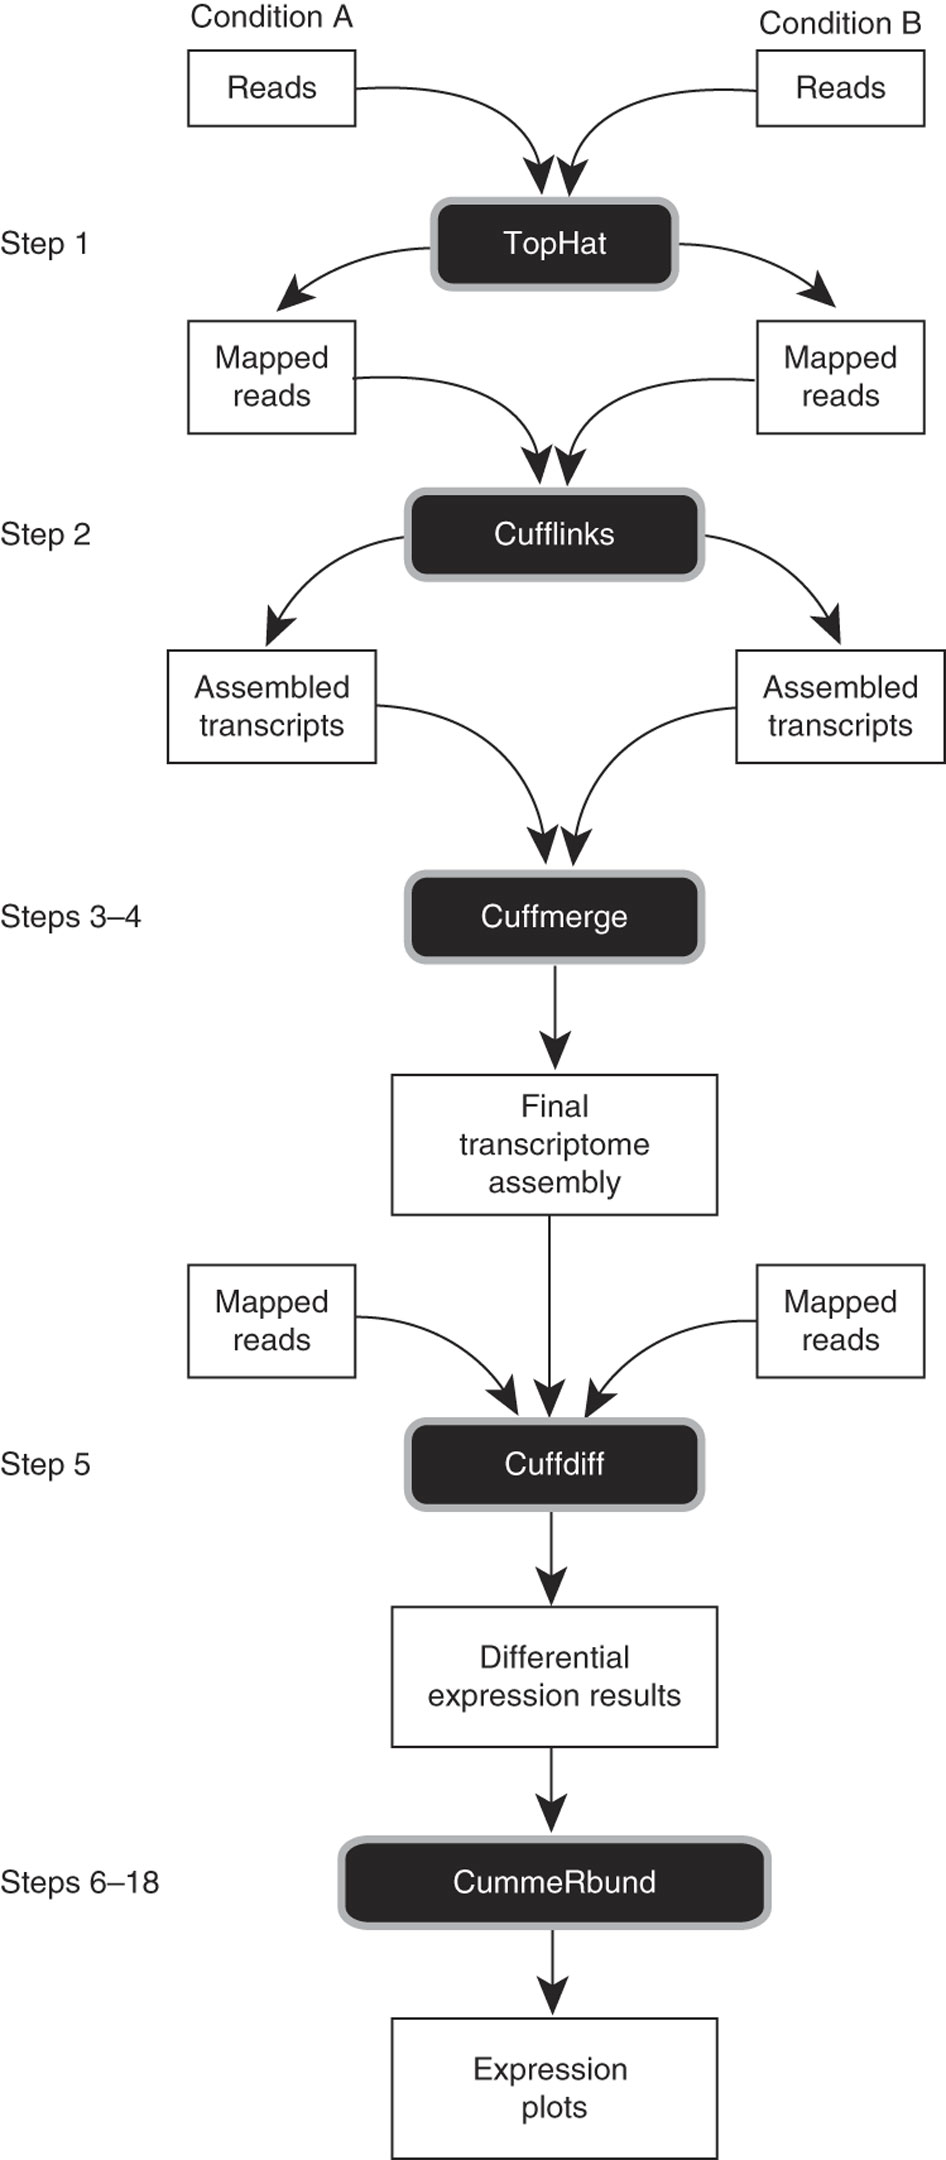
\includegraphics[width=2.8cm]{Images/Tuxedo.jpg}
  \\{\tiny{Trapnell \textit{et al.} (2012), Nature Protocols 7, 562--578}}
\end{columns}
\end{frame}

\begin{frame}
\frametitle{Tophat}
\begin{center}
\begin{enumerate}
\item
Efficient and fast alignment to the genome using bowtie2
\item
Create a data base of putative splice junctions from the reads mapping in step 1
\item
Map reads that did not map in step 1 using the splice information
\end{enumerate}
\end{center}
\end{frame}

\begin{frame}
\frametitle{QC of mapped reads}
\begin{center}
Reads should mostly map to known (annotated genes) \\
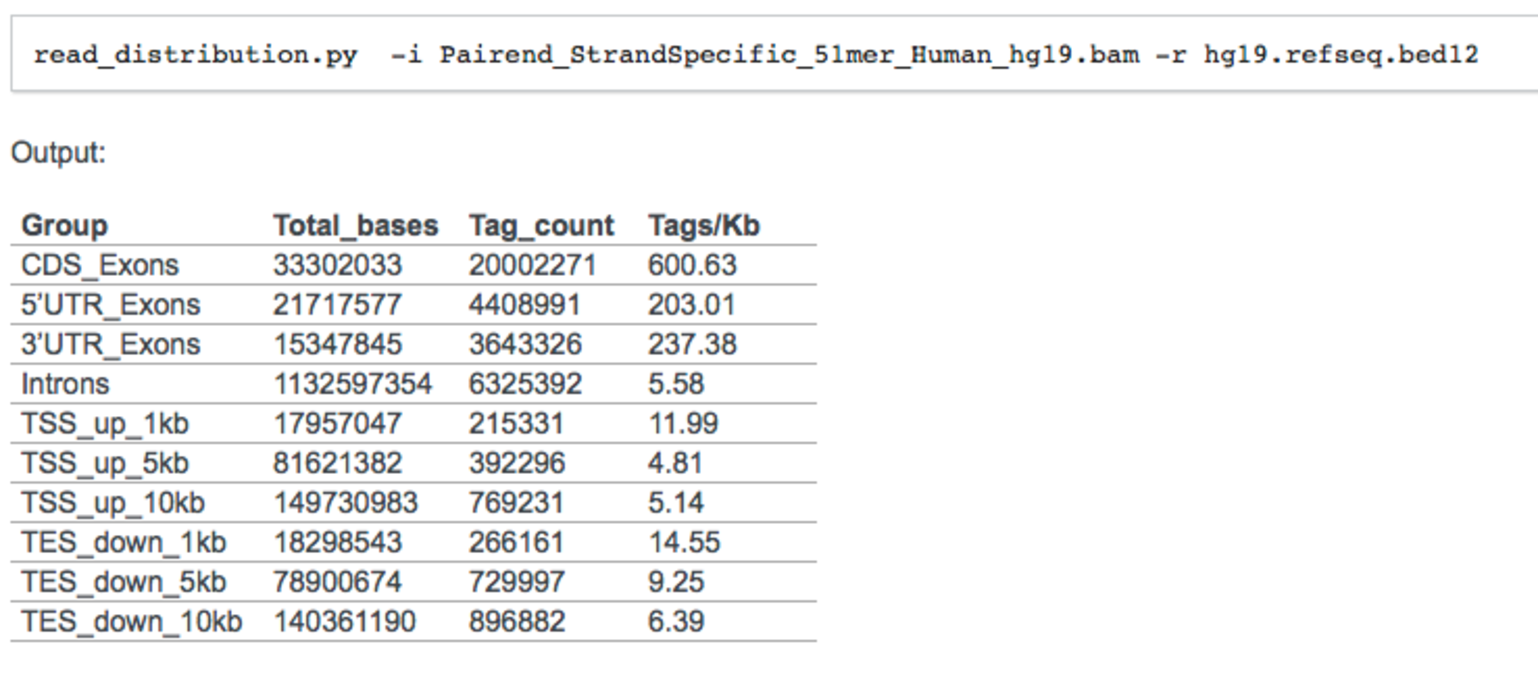
\includegraphics[width=8cm]{Images/read-dist.pdf}
\end{center}
\end{frame}

\begin{frame}
\frametitle{QC of mapped reads}
\begin{center}
Most splice event should be known and canonical (GU-AG)
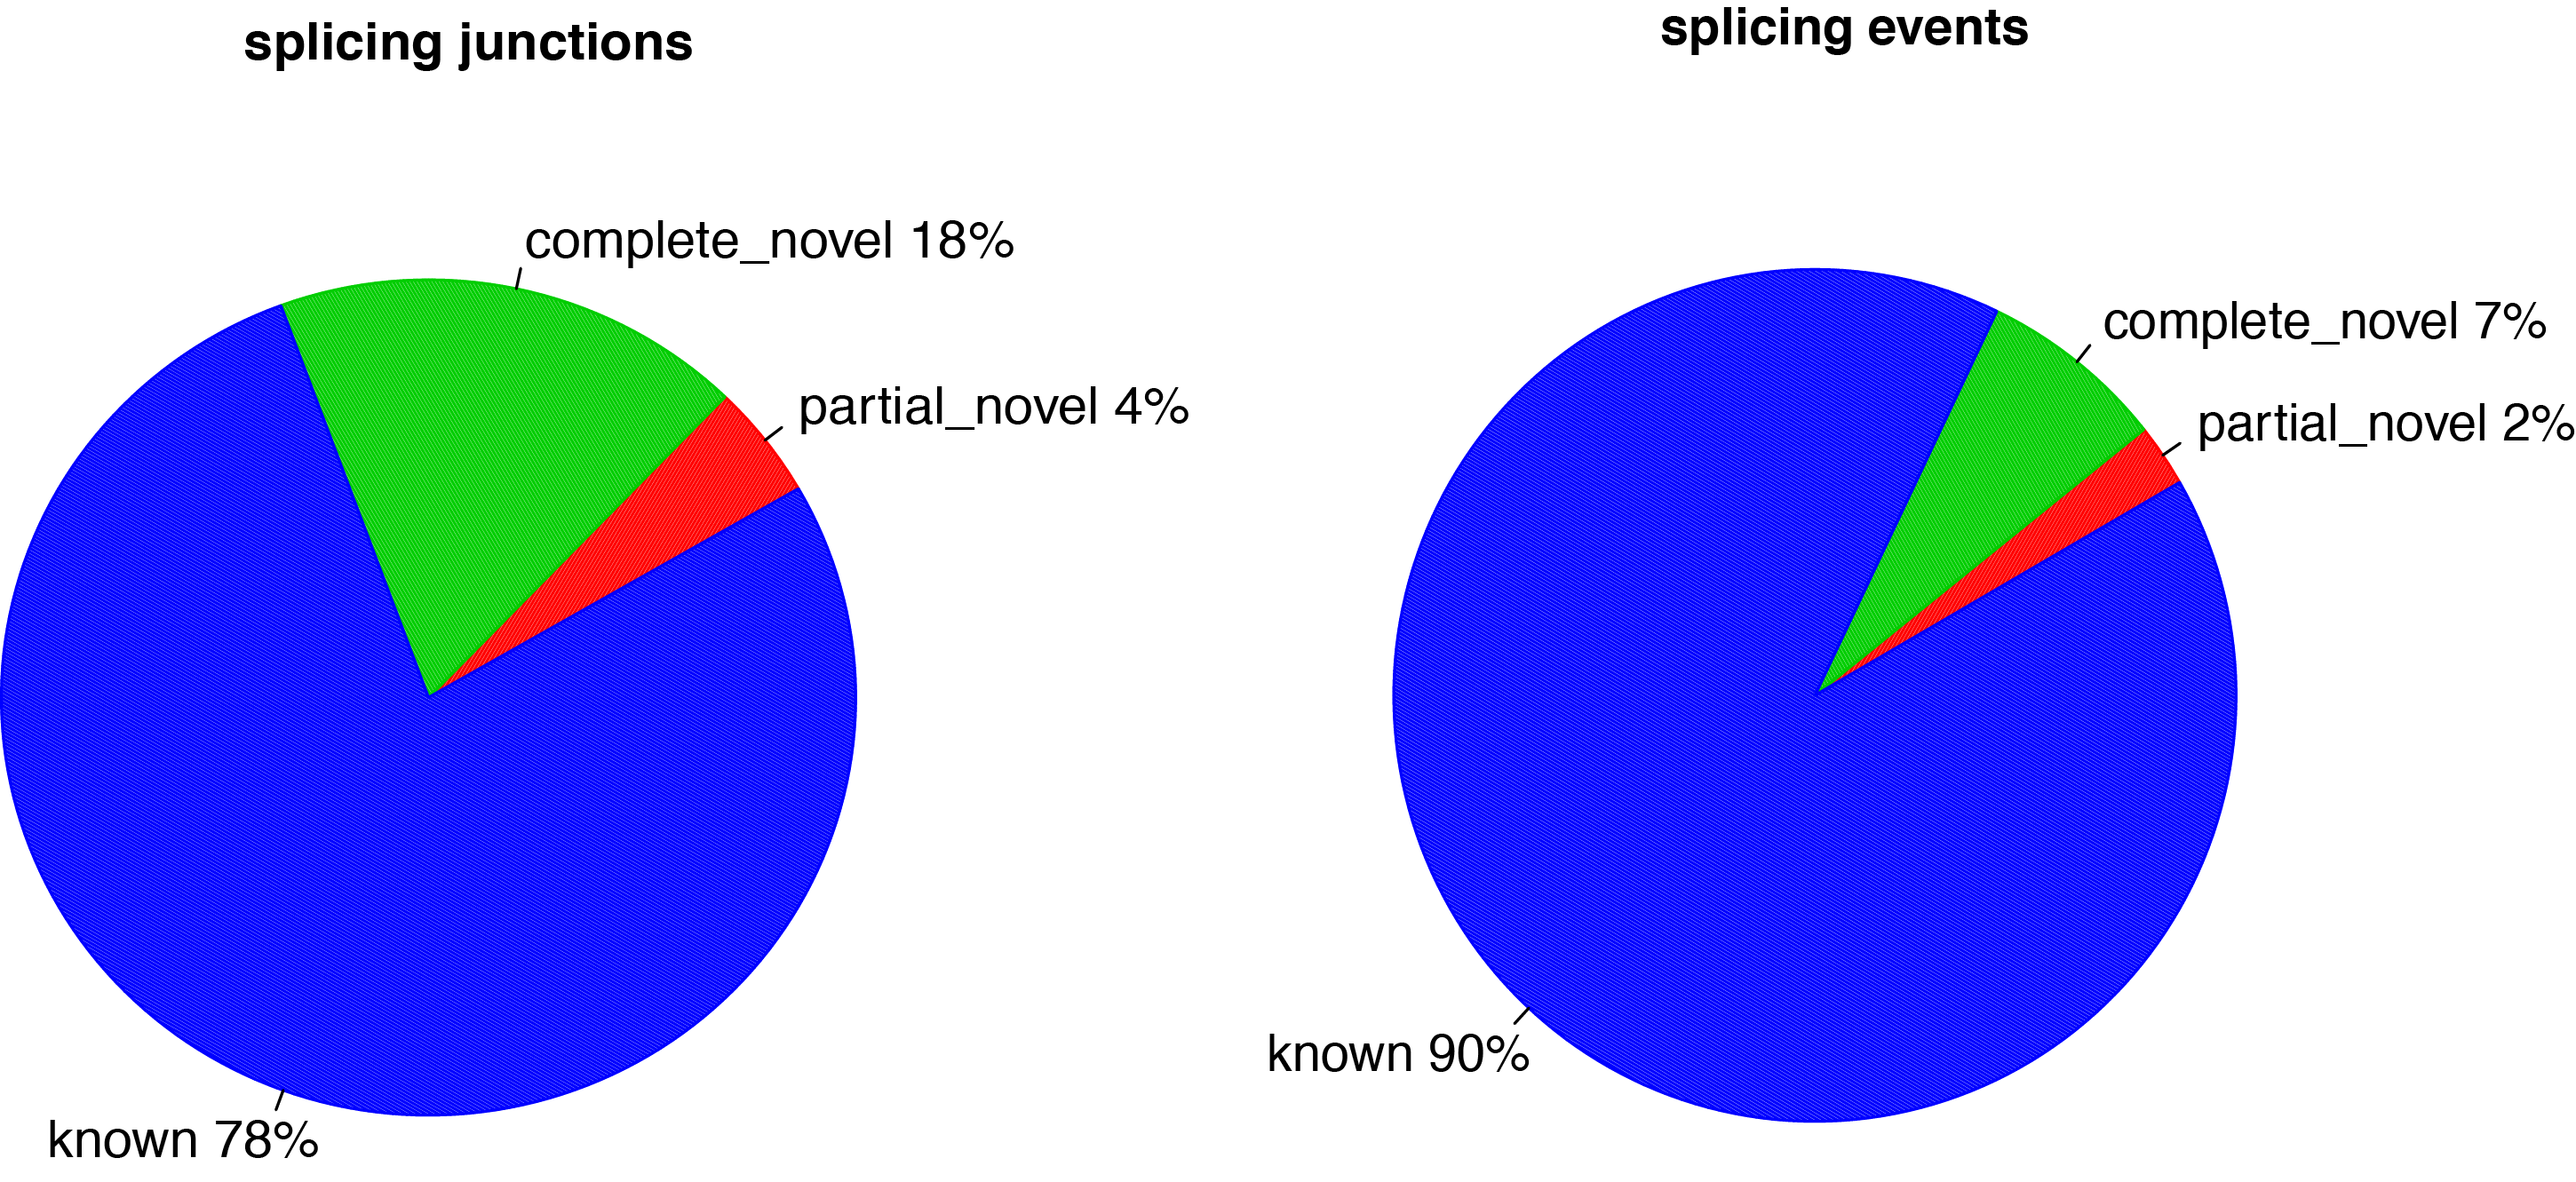
\includegraphics[width=8cm]{Images/junction.png}
\end{center}
\end{frame}

\begin{frame}{Cufflinks}
\begin{center}
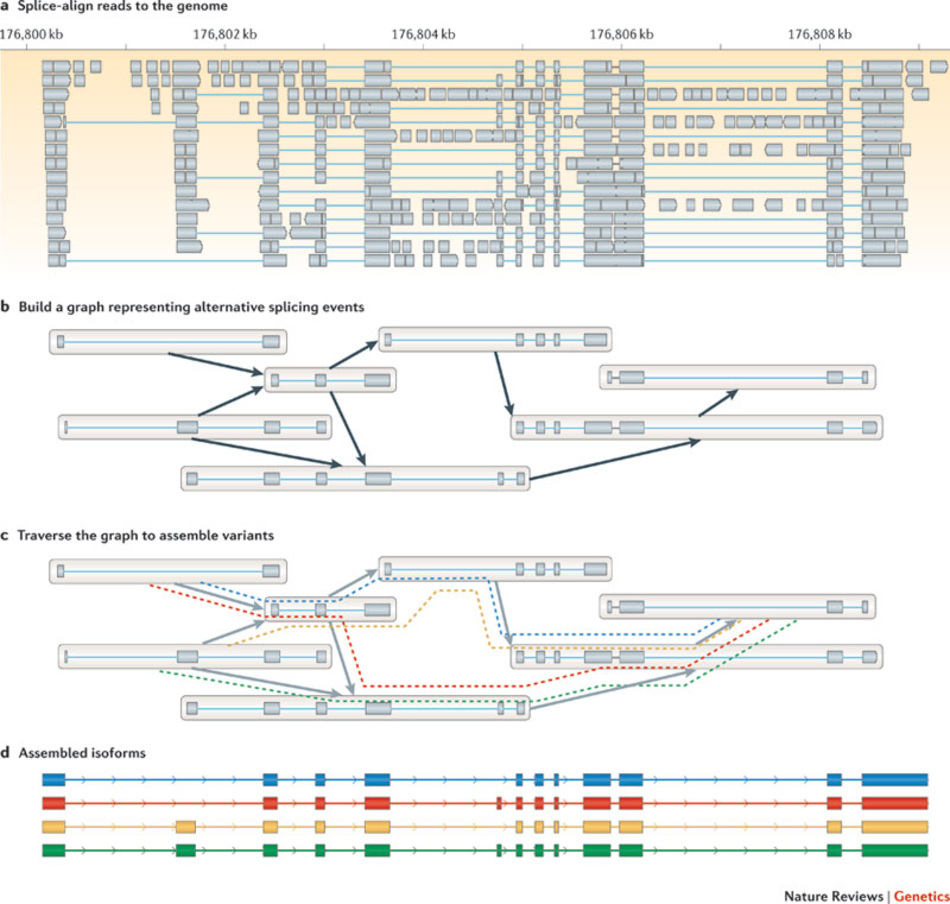
\includegraphics[width=7cm]{Images/Cufflinks-rec.pdf}
\end{center}
\end{frame}

\begin{frame}{Cuffdiff}
\begin{center}
\begin{itemize}
\item
Program that estimate expression levels and identify differentially expressed genes from ngs alignments
\item
Basically uses the read data to estimate dispersion parameters (the amount of deviation from a Poisson distr.)
\item
Genes that show patterns deviating from the above expectations are differentially expressed between treatments
\item
Will work also for detection of isoform differential expression
\end{itemize}
\end{center}
\end{frame}

\subsection{Gene expression from RNA-seq}

\begin{frame}
\frametitle{From counts to gene expression}
\begin{center}
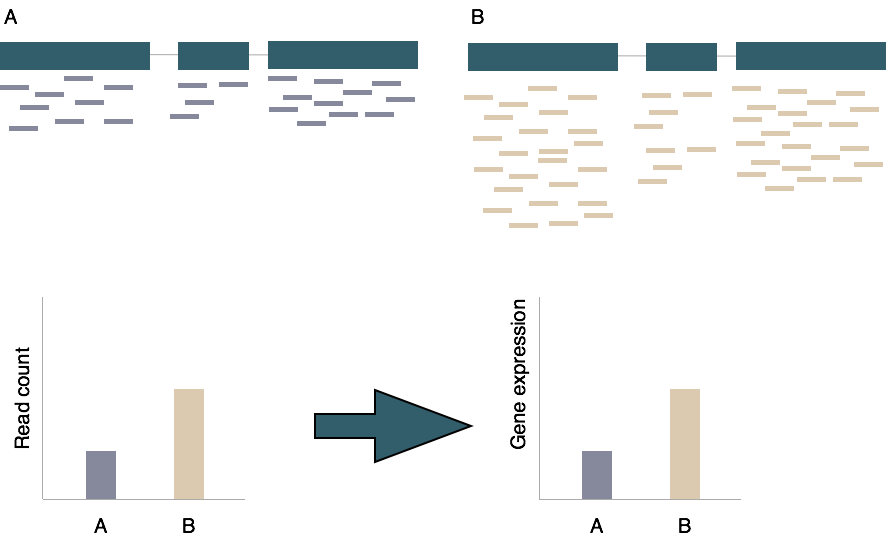
\includegraphics[width=9cm]{Images/Expression1.png}
\end{center}
\end{frame}

\begin{frame}
\frametitle{From counts to gene expression}
\begin{center}
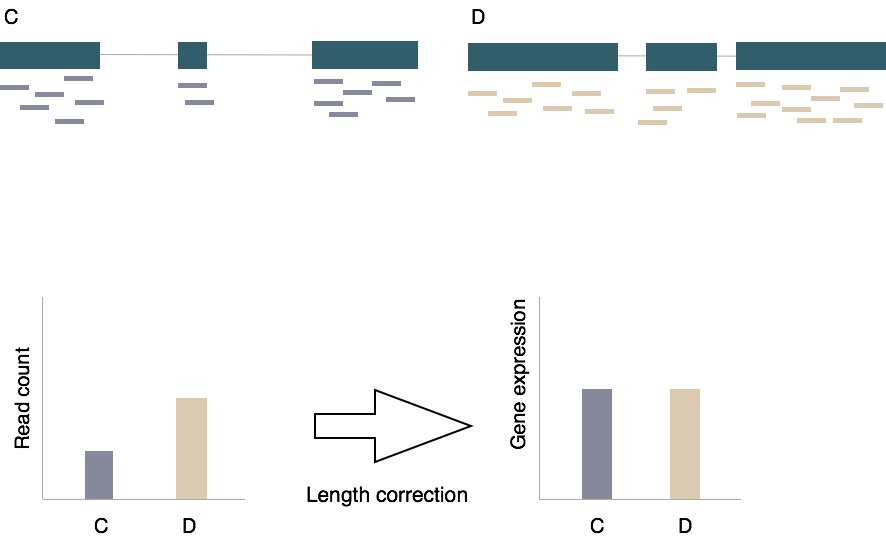
\includegraphics[width=9cm]{Images/Expression2.png}
\end{center}
\end{frame}

\begin{frame}
\frametitle{Not all reads are the same}
\centering
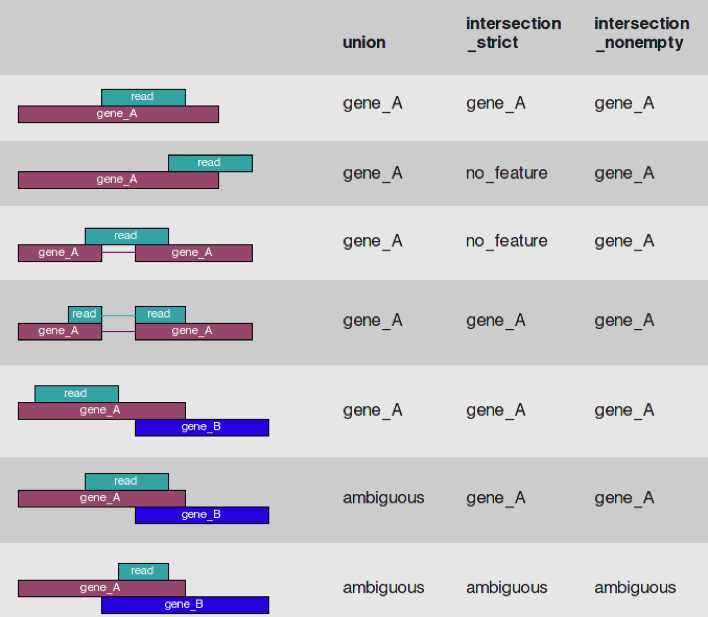
\includegraphics[width=7cm]{Images/HTseq.png}
  \\{\tiny{from: http://www-huber.embl.de/users/anders/HTSeq/doc/count.html}}
\end{frame}

\begin{frame}
\frametitle{Normalized expression Values}
\begin{center}
\begin{itemize}
\item
Mapped read counts are normalized for both length of the transcript they map to and total depth of sequencing.
\item
Count data is hence converted to: Reads/Fragments per kb of transcript length and million mapped reads (RPKM or FPKM)
\end{itemize}
\end{center}
\end{frame}

\begin{frame}
\frametitle{Experimental design}
\begin{center}
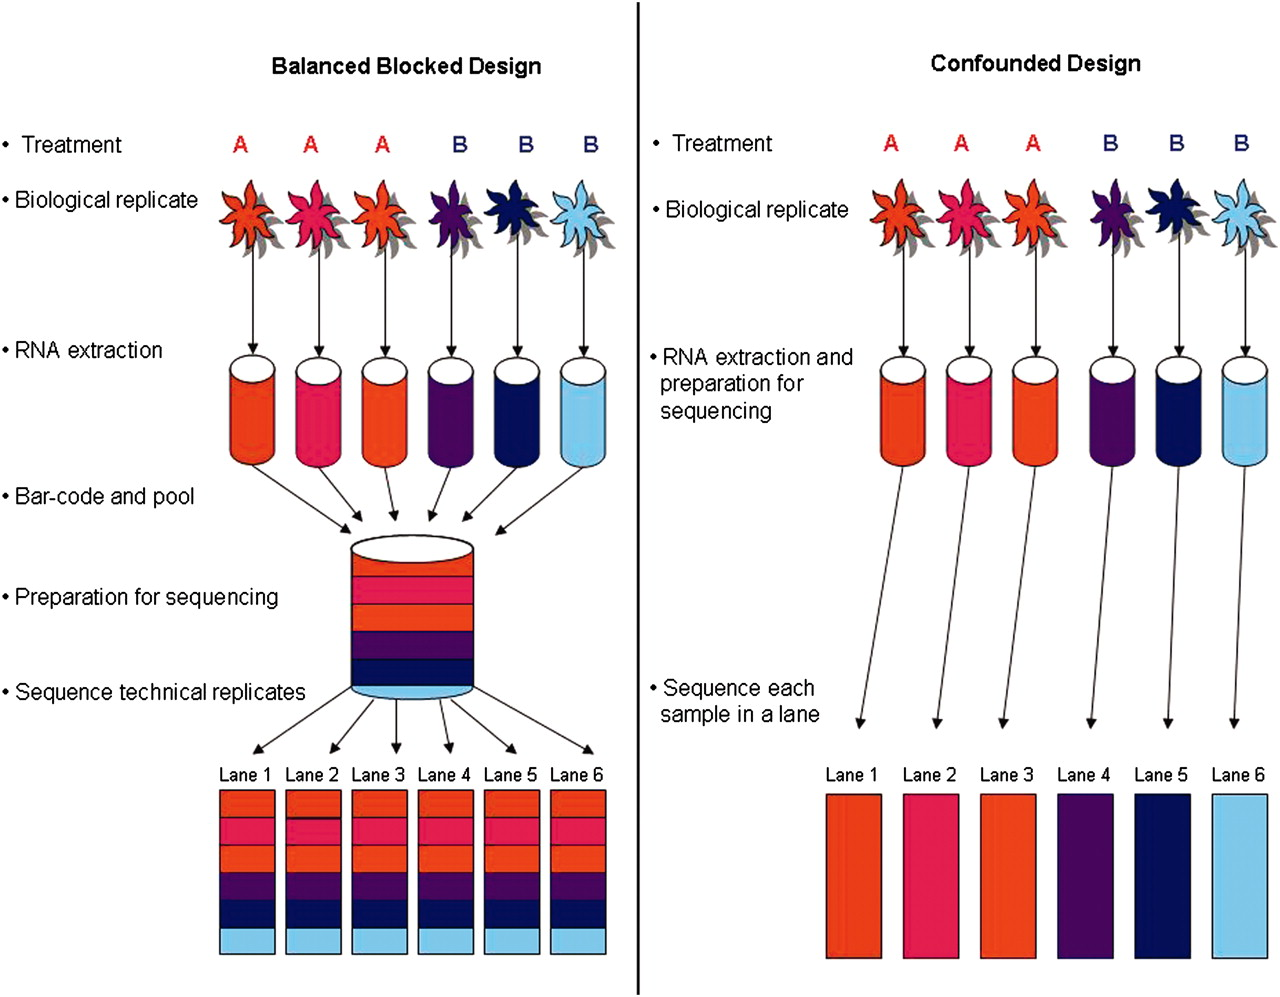
\includegraphics[width=9cm]{Images/BalancedBlock.jpg}
\end{center}
\end{frame}

\begin{frame}
\frametitle{Experimental design}
\begin{center}
\begin{itemize}
\item
Count reads (convert to RPKM/FPKM?)
\item
Small number of reads (= low RPKM/FPKM values) often non-significant
\item
Remember that Fold change is not the same as significance
\end{itemize}
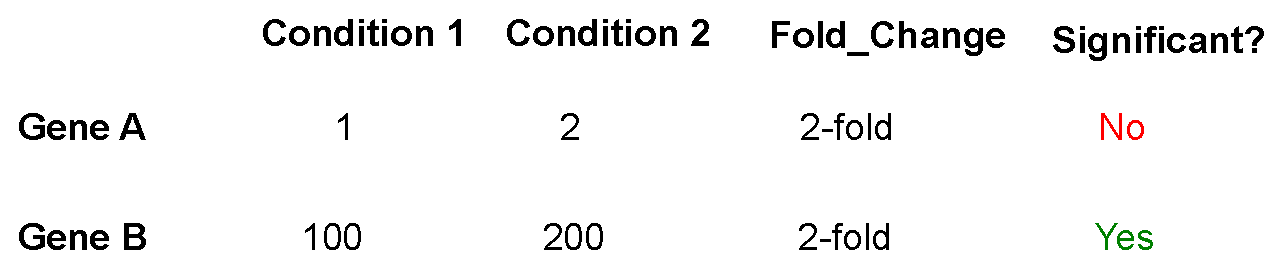
\includegraphics[width=7cm]{Images/FC.pdf}
\end{center}
\end{frame}

\begin{frame}
\frametitle{Two main routes for analysis}
\centering
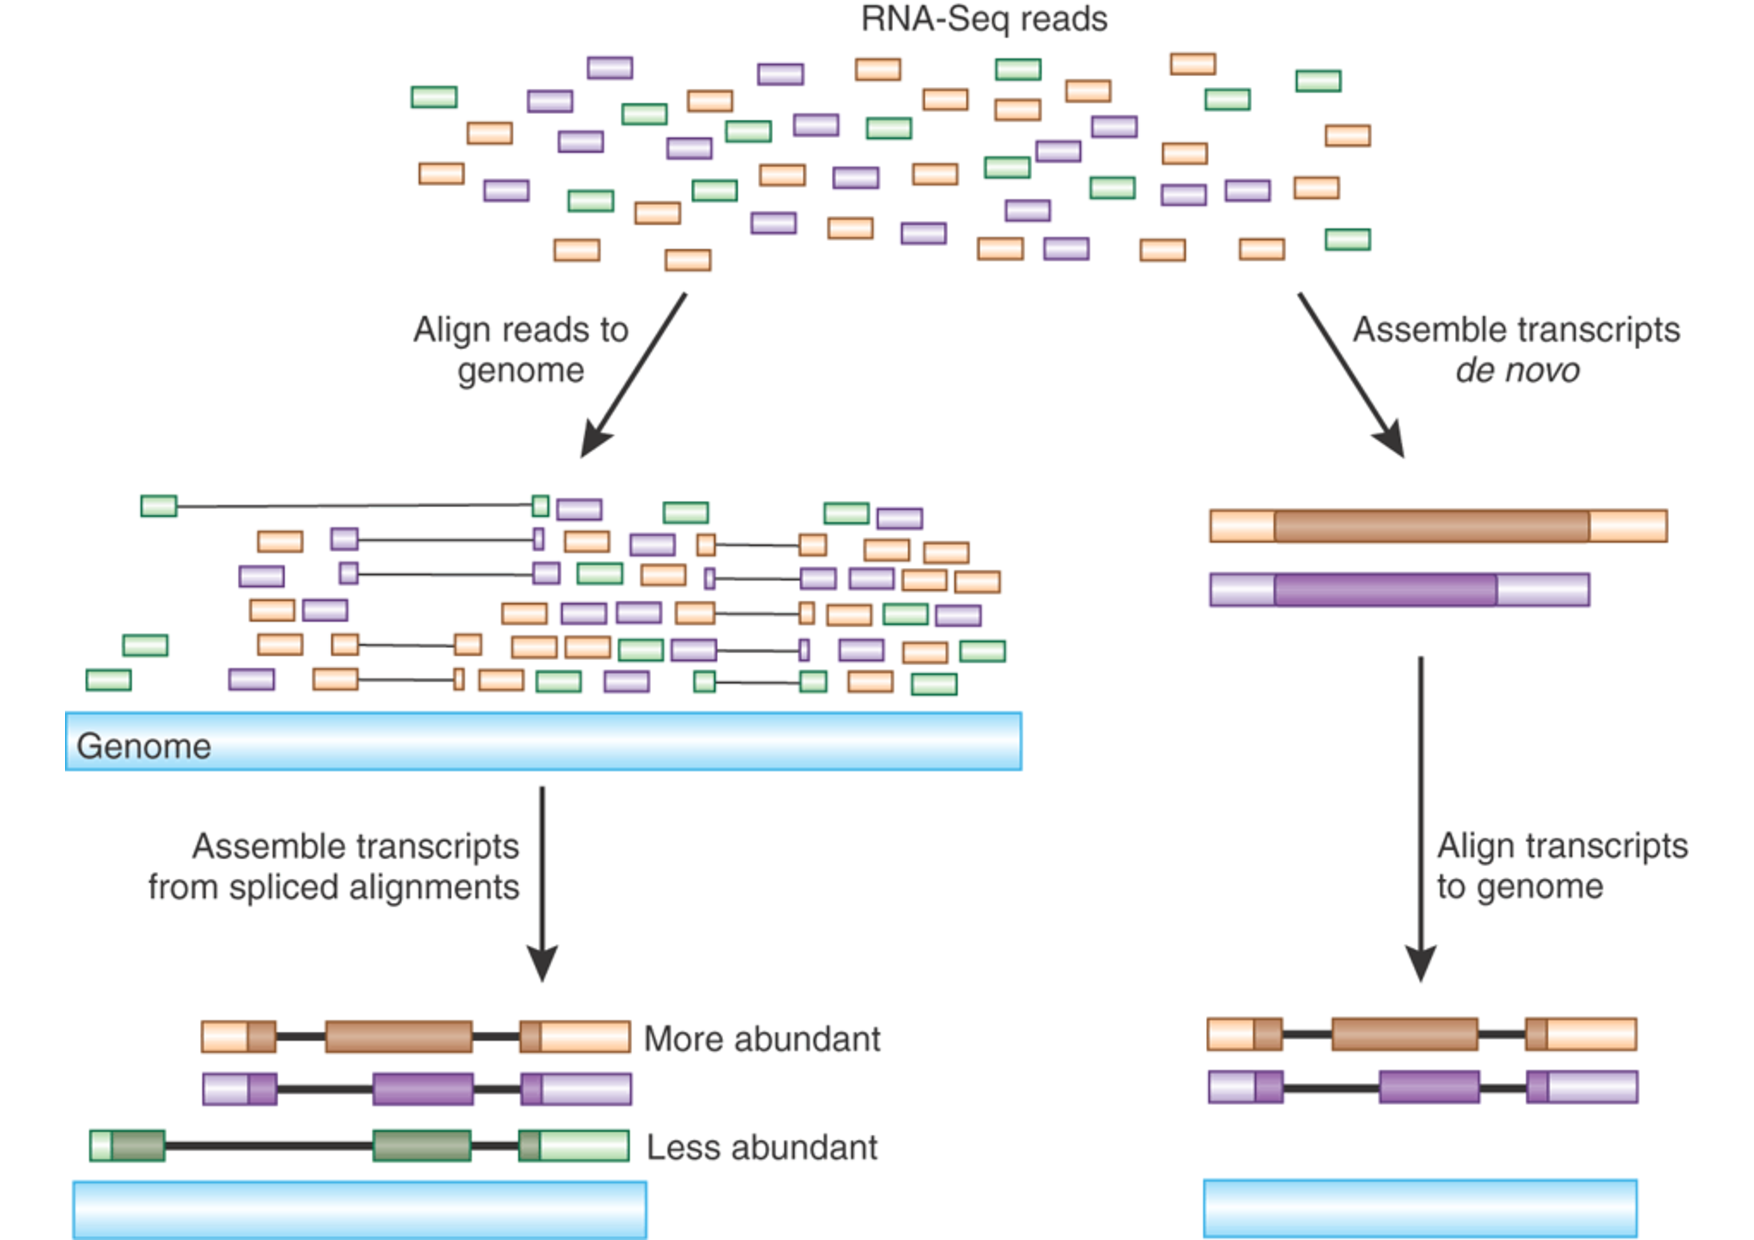
\includegraphics[width=8cm]{Images/advancingRNAseq.pdf}
  \\{\tiny{Haas \& Zody (2010), Nature Biotechnology 28, 421--423}}
\end{frame}

\subsection{de-novo assembly}

\begin{frame}{Major challenges in relation to genome assembly}
\begin{center}
\begin{itemize}
\item
Genes show different levels of gene expression, hence uneven coverage among genes
\item
Many genes are expressed in different isoforms
\item
As sequence depth increase detected number of loci increase. (What is actually expressed?)
\item
Sequence error from highly expressed genes might be seen more often than "true" sequences from lowly expressed genes
\end{itemize}
\end{center}
\end{frame}

\begin{frame}{Several programs available}
\begin{itemize}
\item
SOAP-denovo TRANS
\item
Oases
\item
Trans-ABYSS
\item
Trinity
\end{itemize}
All of them uses de Bruijn graphs to cope with the data and many of them have been developed from a genome assembly program
\end{frame}

\begin{frame}{Trinity }
\begin{center}
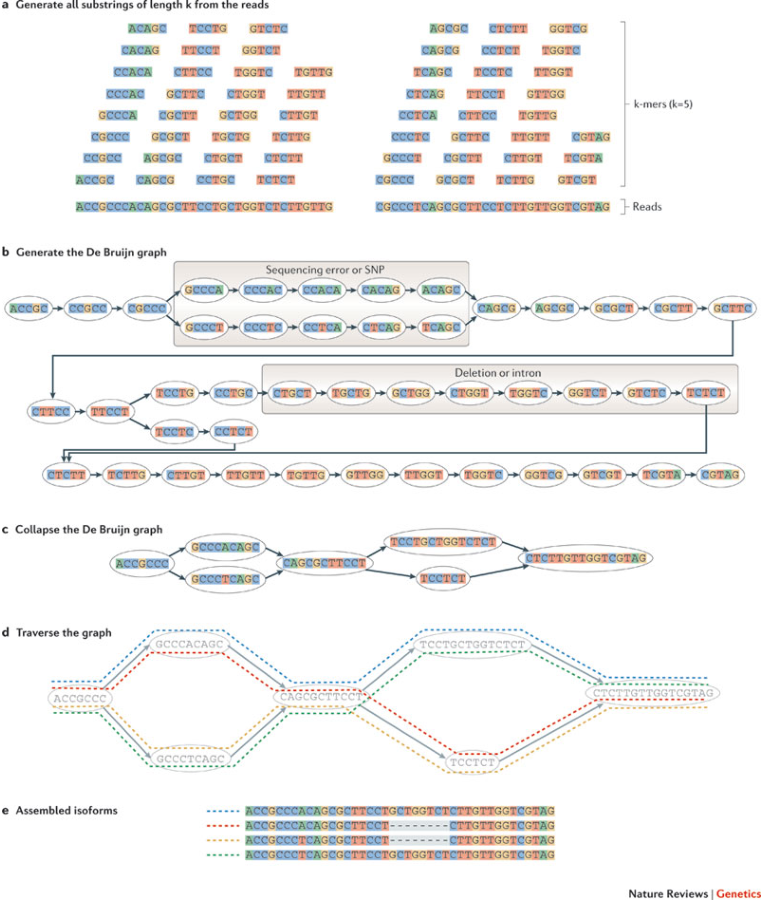
\includegraphics[width=10cm]{Images/denovo.pdf}
\end{center}
\end{frame}

\begin{frame}{Trinity }
\begin{center}
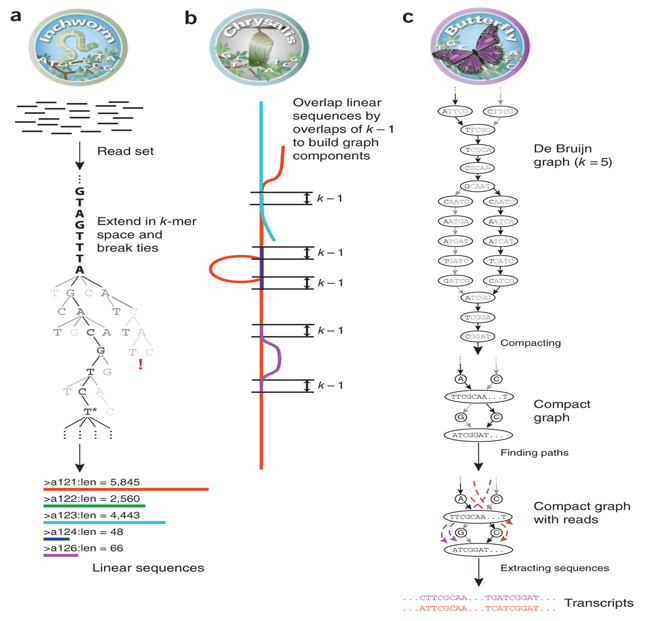
\includegraphics[width=7cm]{Images/Trinity.png}
\end{center}
\end{frame}

\begin{frame}{Summary - with ref.}
\begin{itemize}
\item
Map to genome allow for spliced alignment
\item
If novel transcripts of interest: use method that can re-create transcripts from mapped reads (Cufflinks, Scripture or Bayesembler) \newline
NB! In well annotated genomes most reads should map to known genes
\item
If interest is expression of known genes/exons: Use available annotation for analysis
\item
Spend time on experimental design and more replicates gives more power in gene expression analysis
\end{itemize}
\end{frame}

\begin{frame}{Summary - without ref.}
\begin{itemize}
\item
Assemble using your favourite assembler
\item
Spend lots of time in assessing the results (compare to related species, look for ORFs etc)
\item
Often large number of partial transcripts (hence often large number of contigs).
\item
Merge with other data from transcripts?
\end{itemize}
\end{frame}


\end{document}
\message{ !name(RNA-seq_intro.tex) !offset(-450) }
